% !TEX root = ../main.tex
\section{Testing and Validation}

We ran the notebook end to end on three file pairs (spec §8.2). For each run, the configuration is
the content of the two input files, shown as a screenshot of the files as read from disk. The output
is shown in three screenshots of the notebook cell: the parsed grid with the CSP schedule and its
constraint check, then the integration output for UCS, then for \astar.

\subsection{Test run 1: our files (\code{Environment.txt}, \code{Schedule.txt})}
The schedule is D1\dots D5 in T1\dots T5, with T6 empty, and all constraints are satisfied. Both
algorithms clean all five cells and return to the charger: 64 moves, cost 64, status SUCCESS.

\figcenterbegin
\begin{figure}[H]
\centering
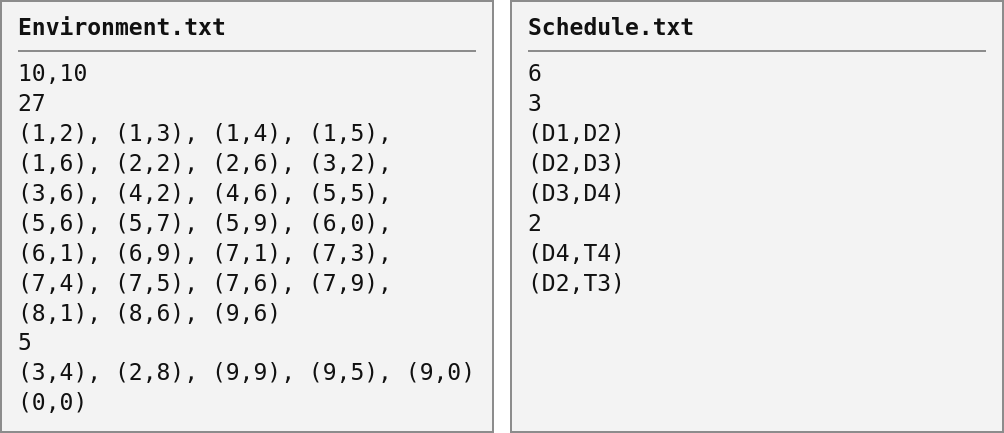
\includegraphics[width=0.8\linewidth]{run1_config.png}
\caption{Test run 1 (own files): configuration, the environment and schedule input files.}
\label{fig:run1-config}
\end{figure}
\figcenterend

\figcenterbegin
\begin{figure}[H]
\centering
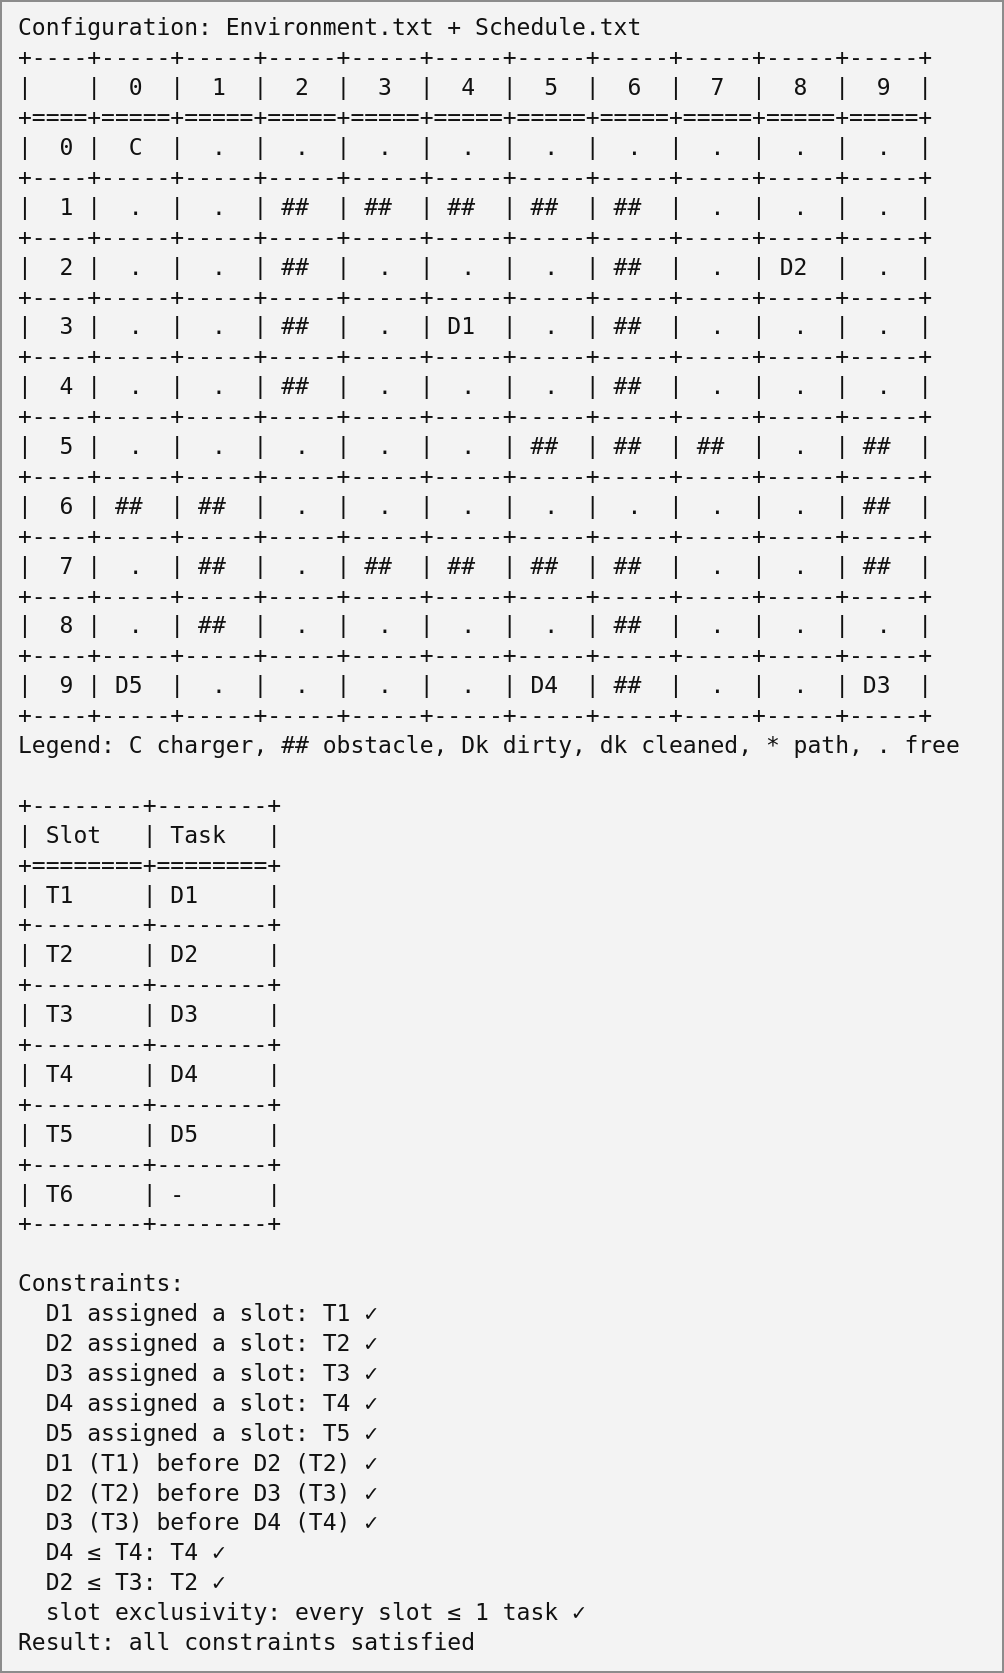
\includegraphics[width=0.8\linewidth]{run1_schedule.png}
\caption{Test run 1 (own files): parsed grid, CSP schedule and constraint check.}
\label{fig:run1-schedule}
\end{figure}
\figcenterend

\figcenterbegin
\begin{figure}[H]
\centering
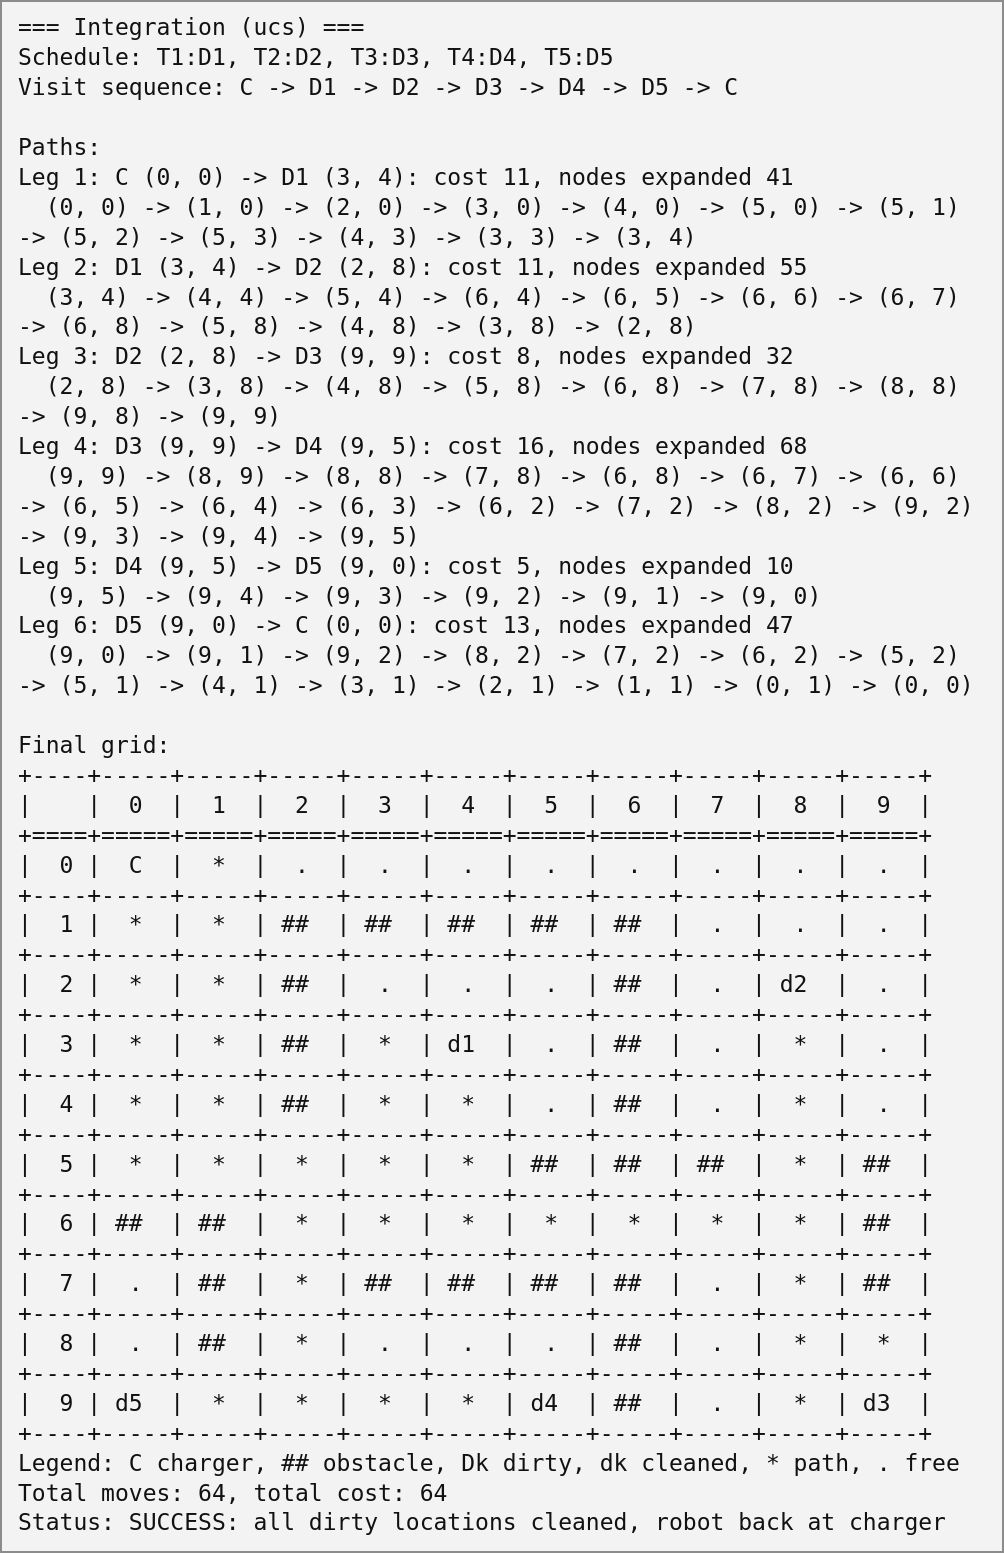
\includegraphics[width=0.8\linewidth]{run1_ucs.png}
\caption{Test run 1 (own files): integration output with UCS.}
\label{fig:run1-ucs}
\end{figure}
\figcenterend

\figcenterbegin
\begin{figure}[H]
\centering
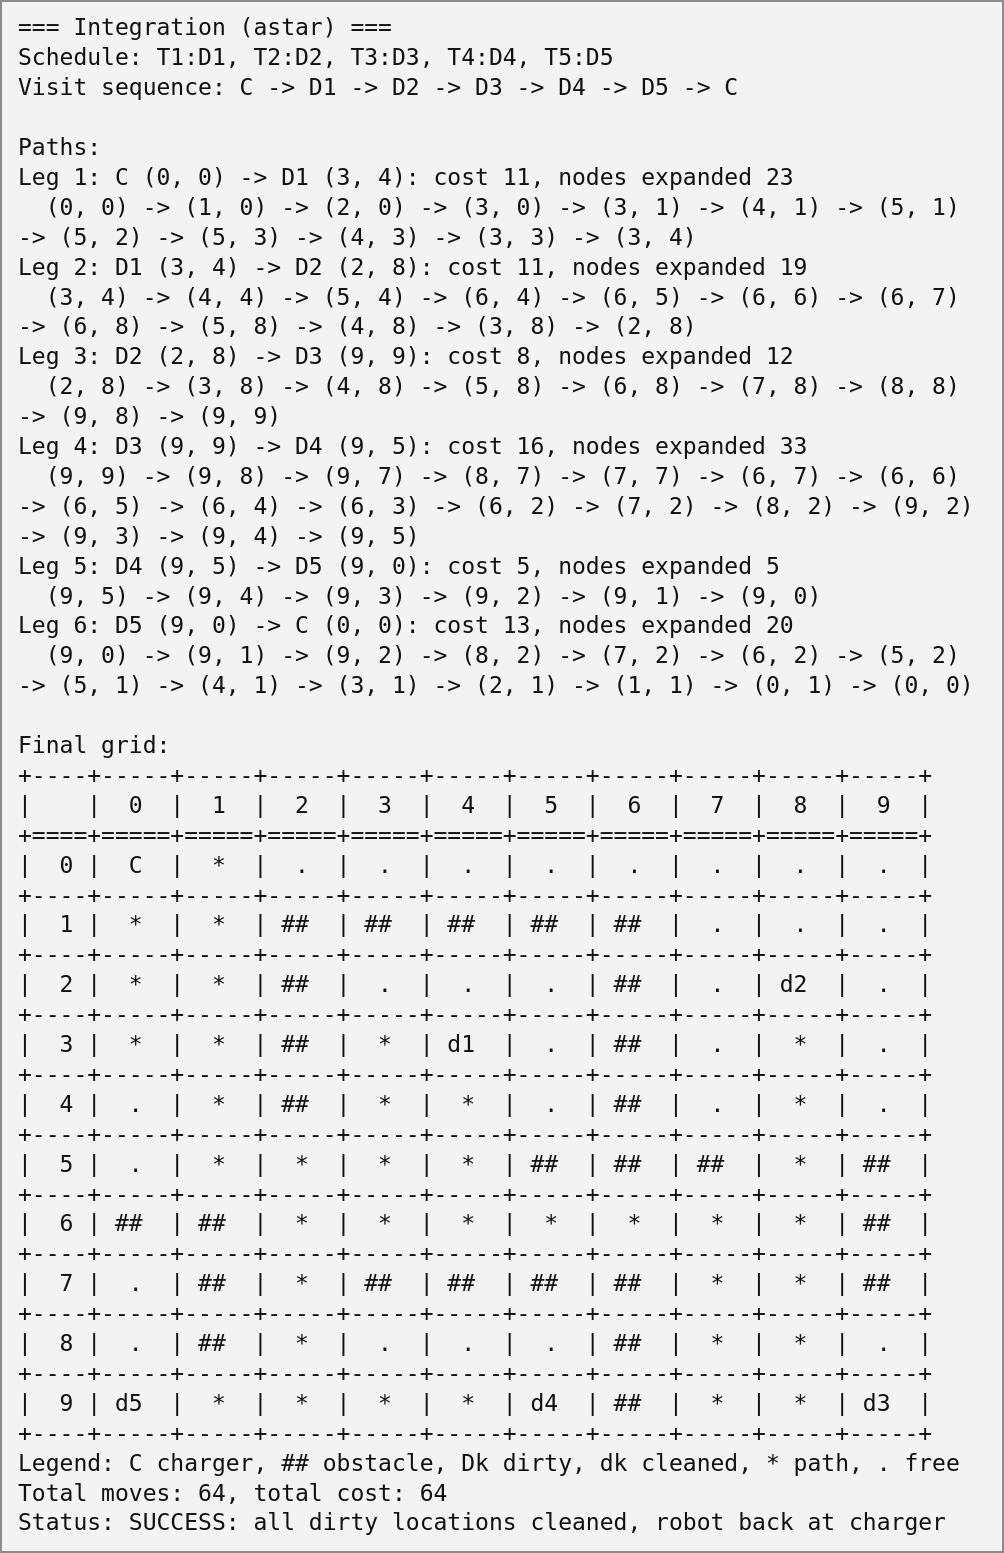
\includegraphics[width=0.8\linewidth]{run1_astar.png}
\caption{Test run 1 (own files): integration output with \astar.}
\label{fig:run1-astar}
\end{figure}
\figcenterend


\newpage
\subsection{Test run 2: provided sample (\code{Environment\_Sample.txt}, \code{Schedule\_Sample.txt})}
The schedule is T1:D2, T2:D1, T3:D3, T4:D4, and all constraints are satisfied. Both algorithms
finish with 34 moves, cost 34, status SUCCESS.

\figcenterbegin
\begin{figure}[H]
\centering
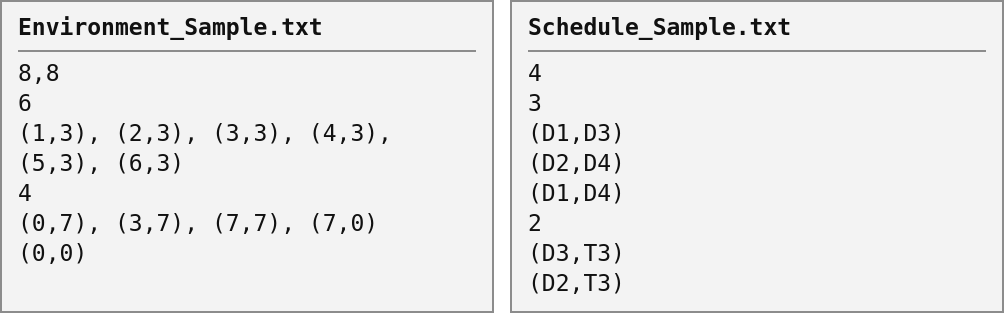
\includegraphics[width=0.8\linewidth]{run2_config.png}
\caption{Test run 2 (sample files): configuration, the environment and schedule input files.}
\label{fig:run2-config}
\end{figure}
\figcenterend

\figcenterbegin
\begin{figure}[H]
\centering
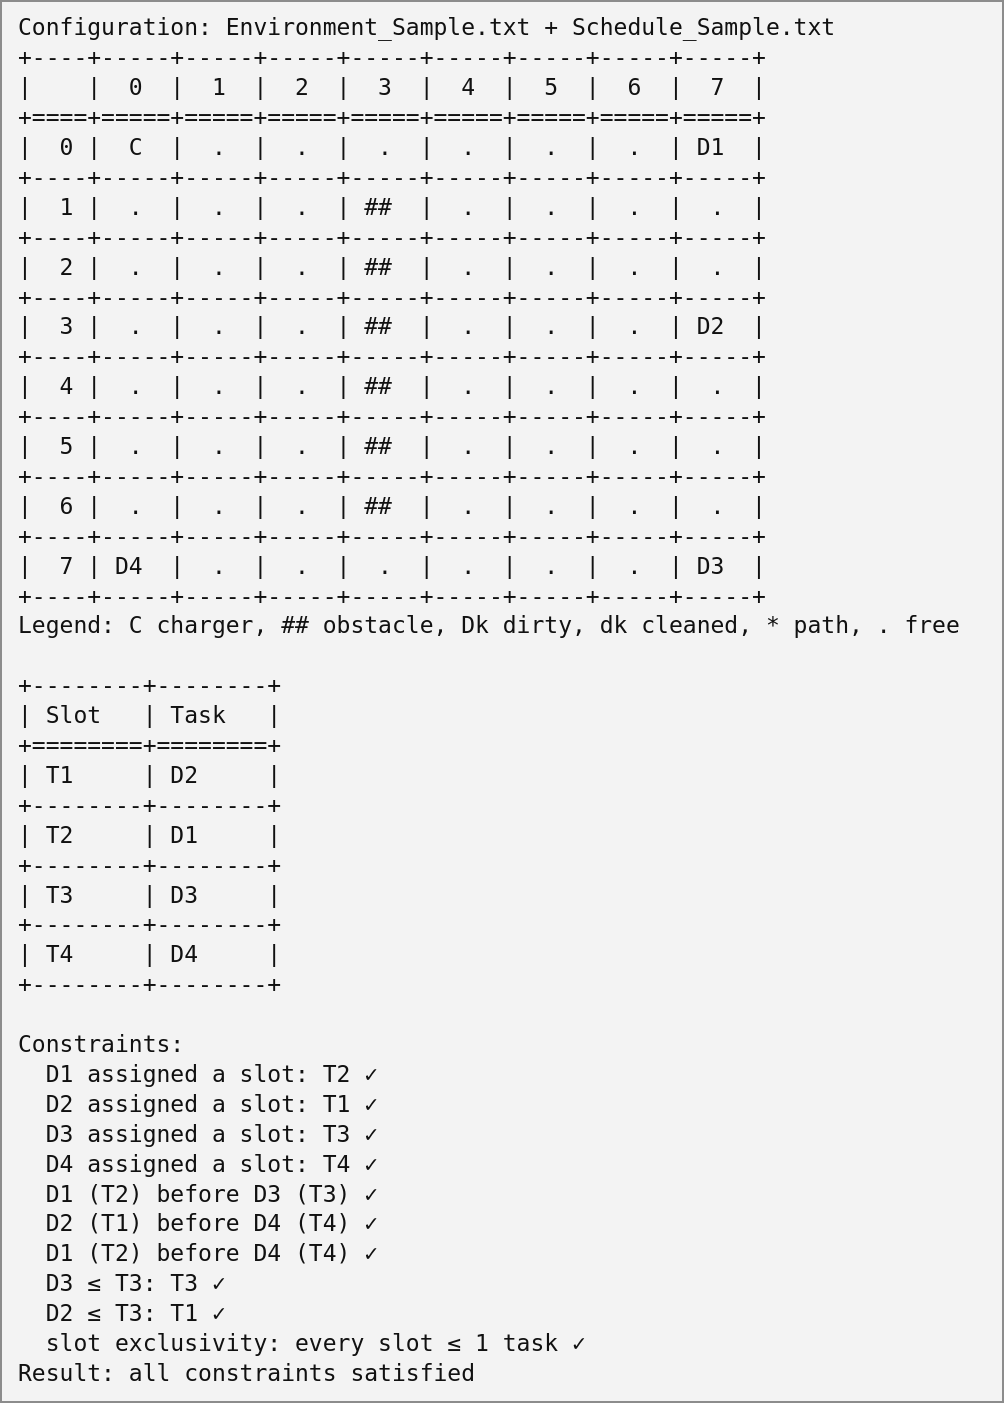
\includegraphics[width=0.8\linewidth]{run2_schedule.png}
\caption{Test run 2 (sample files): parsed grid, CSP schedule and constraint check.}
\label{fig:run2-schedule}
\end{figure}
\figcenterend

\figcenterbegin
\begin{figure}[H]
\centering
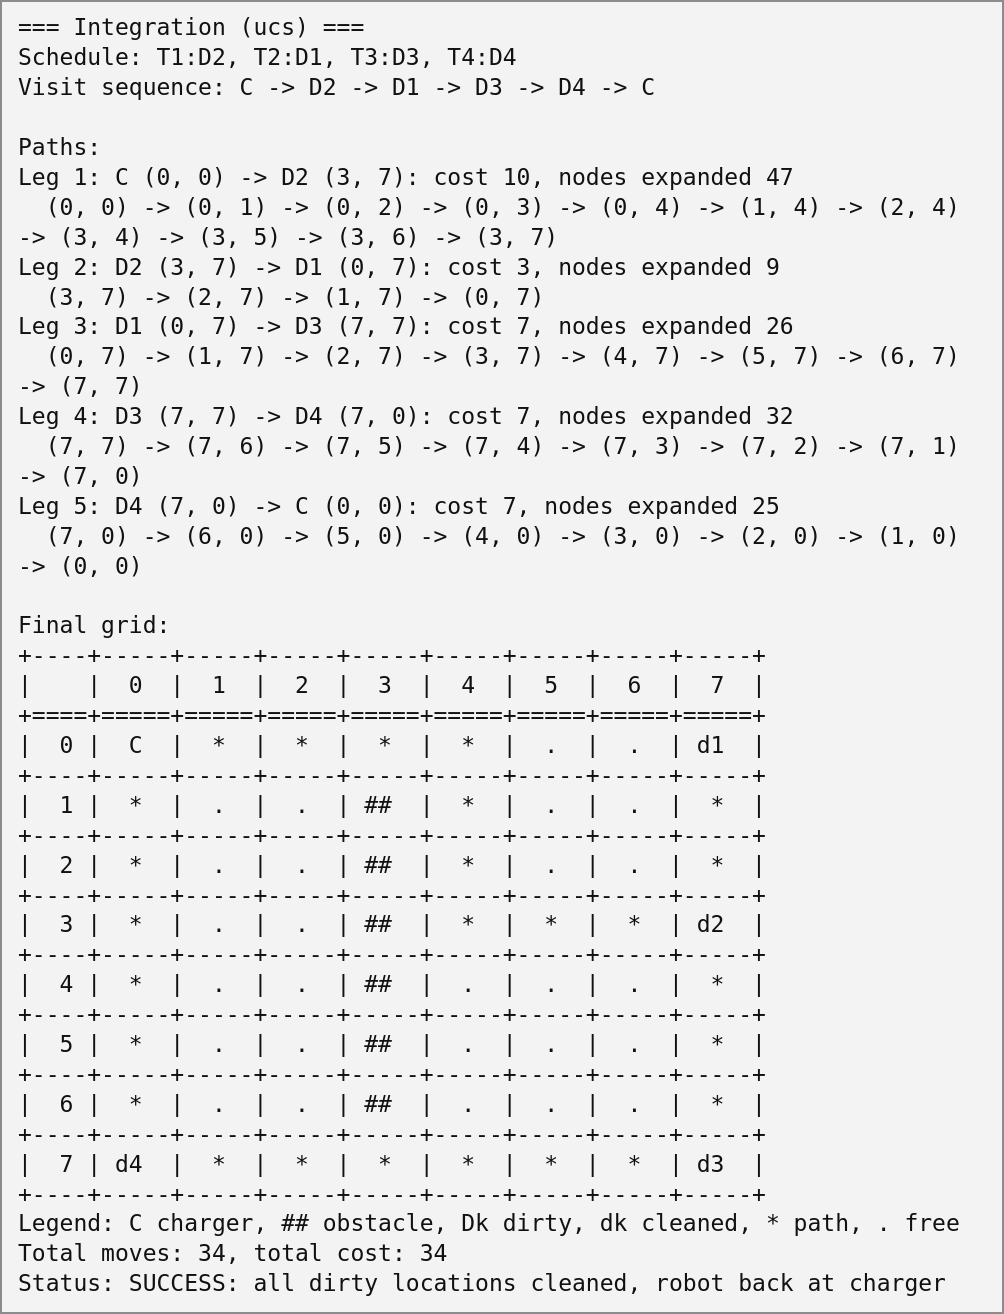
\includegraphics[width=0.8\linewidth]{run2_ucs.png}
\caption{Test run 2 (sample files): integration output with UCS.}
\label{fig:run2-ucs}
\end{figure}
\figcenterend

\figcenterbegin
\begin{figure}[H]
\centering
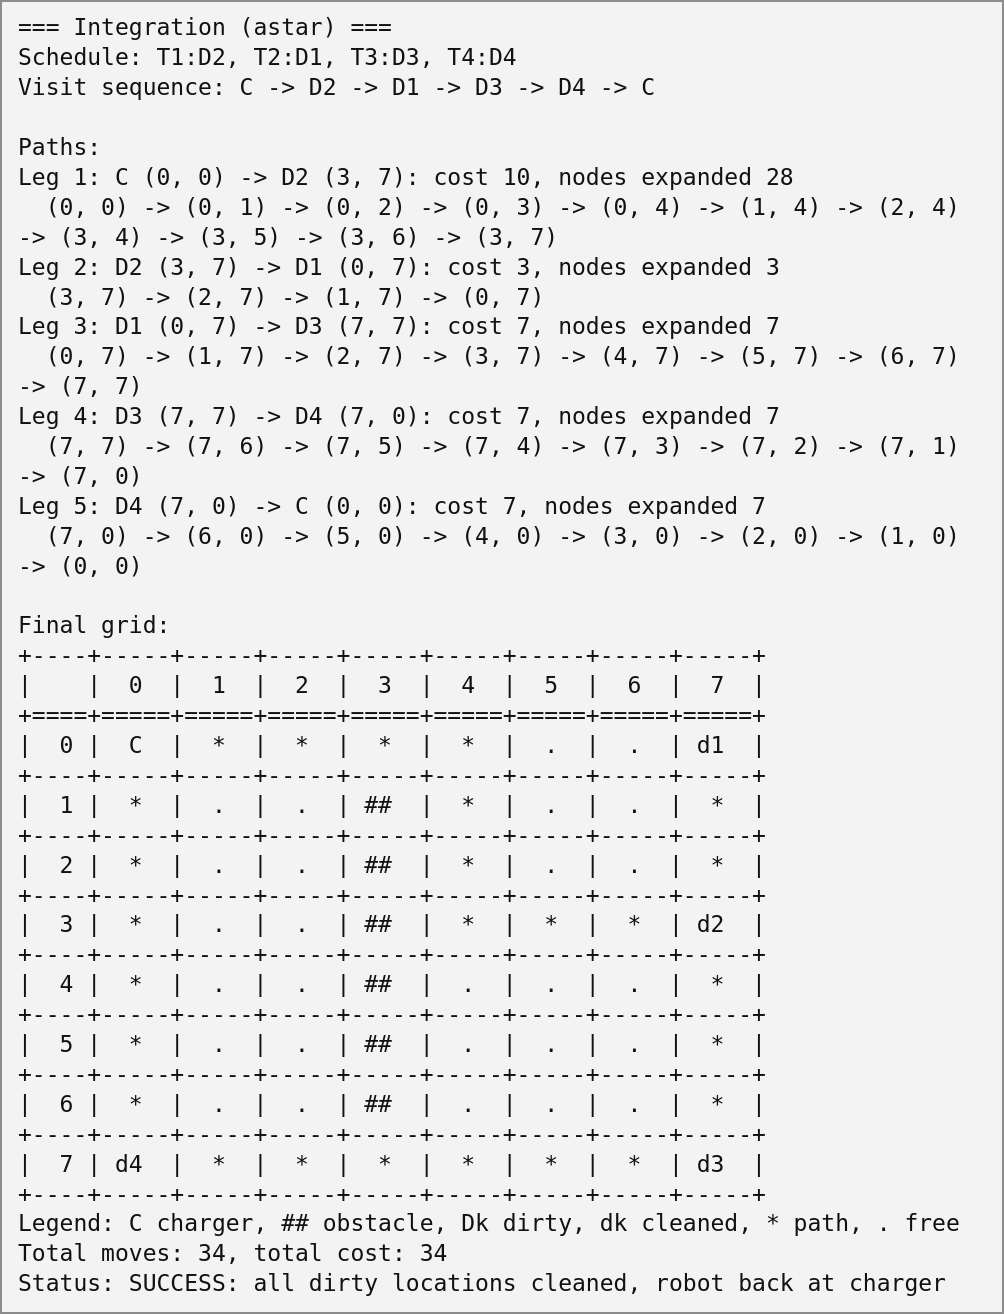
\includegraphics[width=0.8\linewidth]{run2_astar.png}
\caption{Test run 2 (sample files): integration output with \astar.}
\label{fig:run2-astar}
\end{figure}
\figcenterend

\newpage
\subsection{Test run 3: failure case (\code{Environment\_Error.txt}, \code{Schedule\_Error.txt})}
This is our environment with two extra obstacles at (8,0) and (9,1), which wall in D5 at (9,0).
The schedule is unchanged and still feasible, so the CSP succeeds. The leg D4$\to$D5 then returns no
path (69 nodes expanded). The system stops there and prints
\code{FAILURE: no path from D4 (9, 5) to D5 (9, 0)}, lists D1--D4 as cleaned and D5 as not cleaned,
and states that the robot did not return to the charger. The final grid shows D5 still dirty
(Figures~\ref{fig:run3-ucs} and~\ref{fig:run3-astar}).

\figcenterbegin
\begin{figure}[H]
\centering
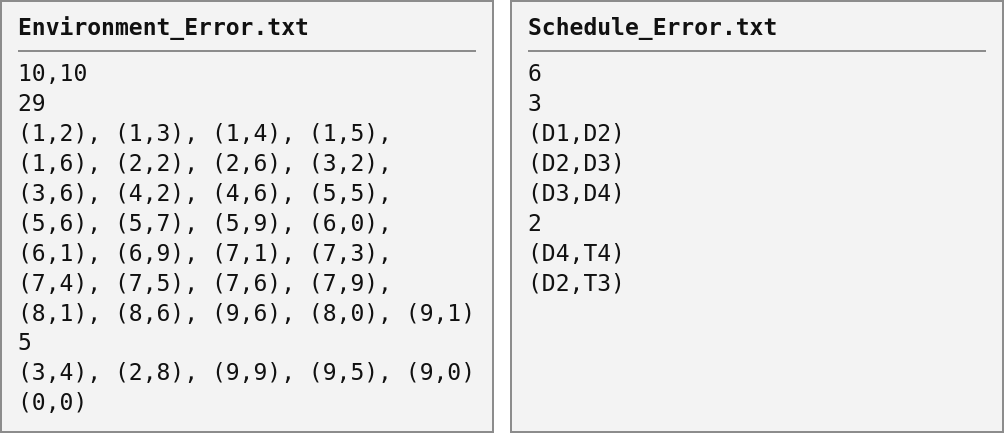
\includegraphics[width=0.8\linewidth]{run3_config.png}
\caption{Test run 3 (error files): configuration, the environment and schedule input files.}
\label{fig:run3-config}
\end{figure}
\figcenterend

\figcenterbegin
\begin{figure}[H]
\centering
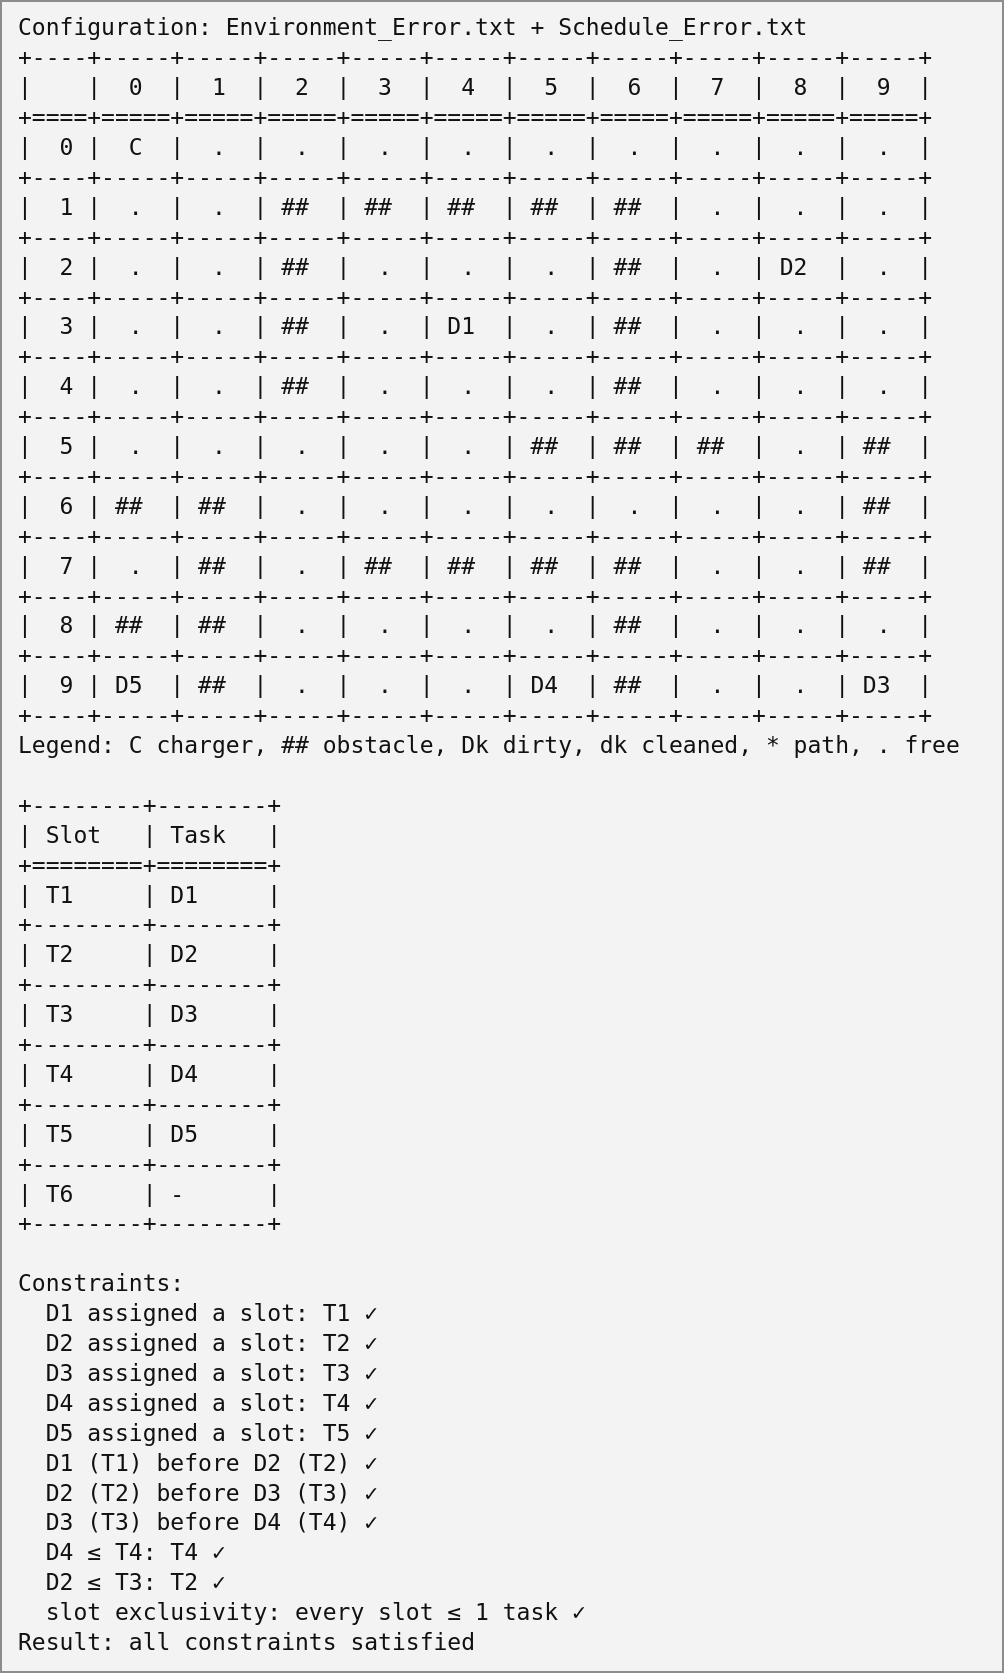
\includegraphics[width=0.8\linewidth]{run3_schedule.png}
\caption{Test run 3 (error files): parsed grid, CSP schedule and constraint check.}
\label{fig:run3-schedule}
\end{figure}
\figcenterend

\figcenterbegin
\begin{figure}[H]
\centering
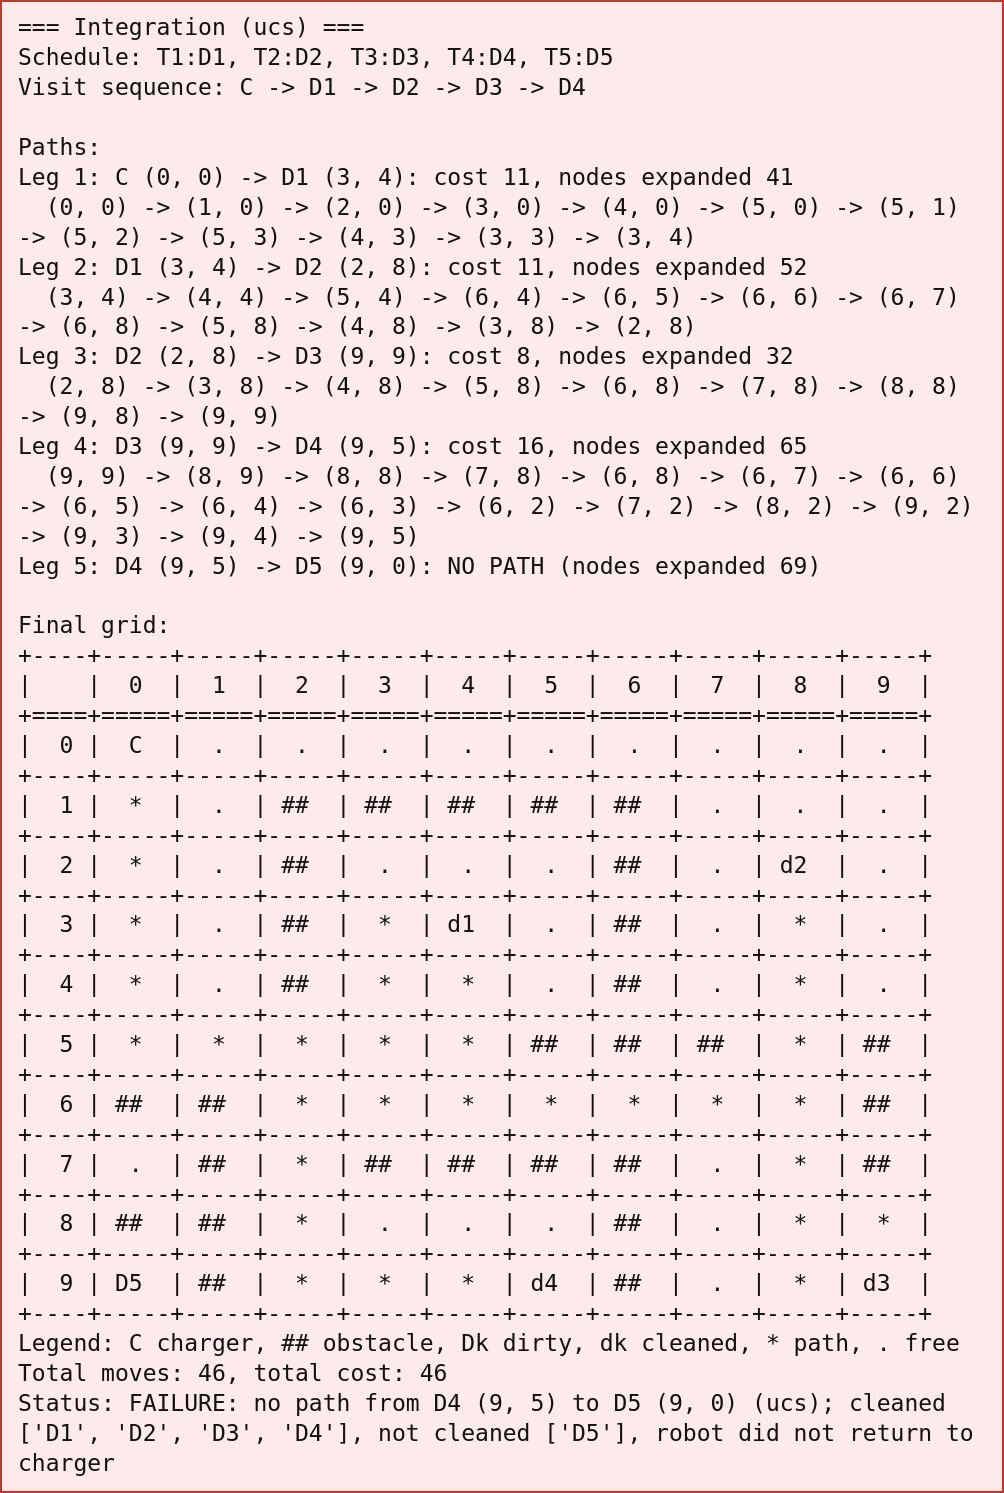
\includegraphics[width=0.8\linewidth]{run3_ucs.png}
\caption{Test run 3 (error files): integration output with UCS.}
\label{fig:run3-ucs}
\end{figure}
\figcenterend

\figcenterbegin
\begin{figure}[H]
\centering
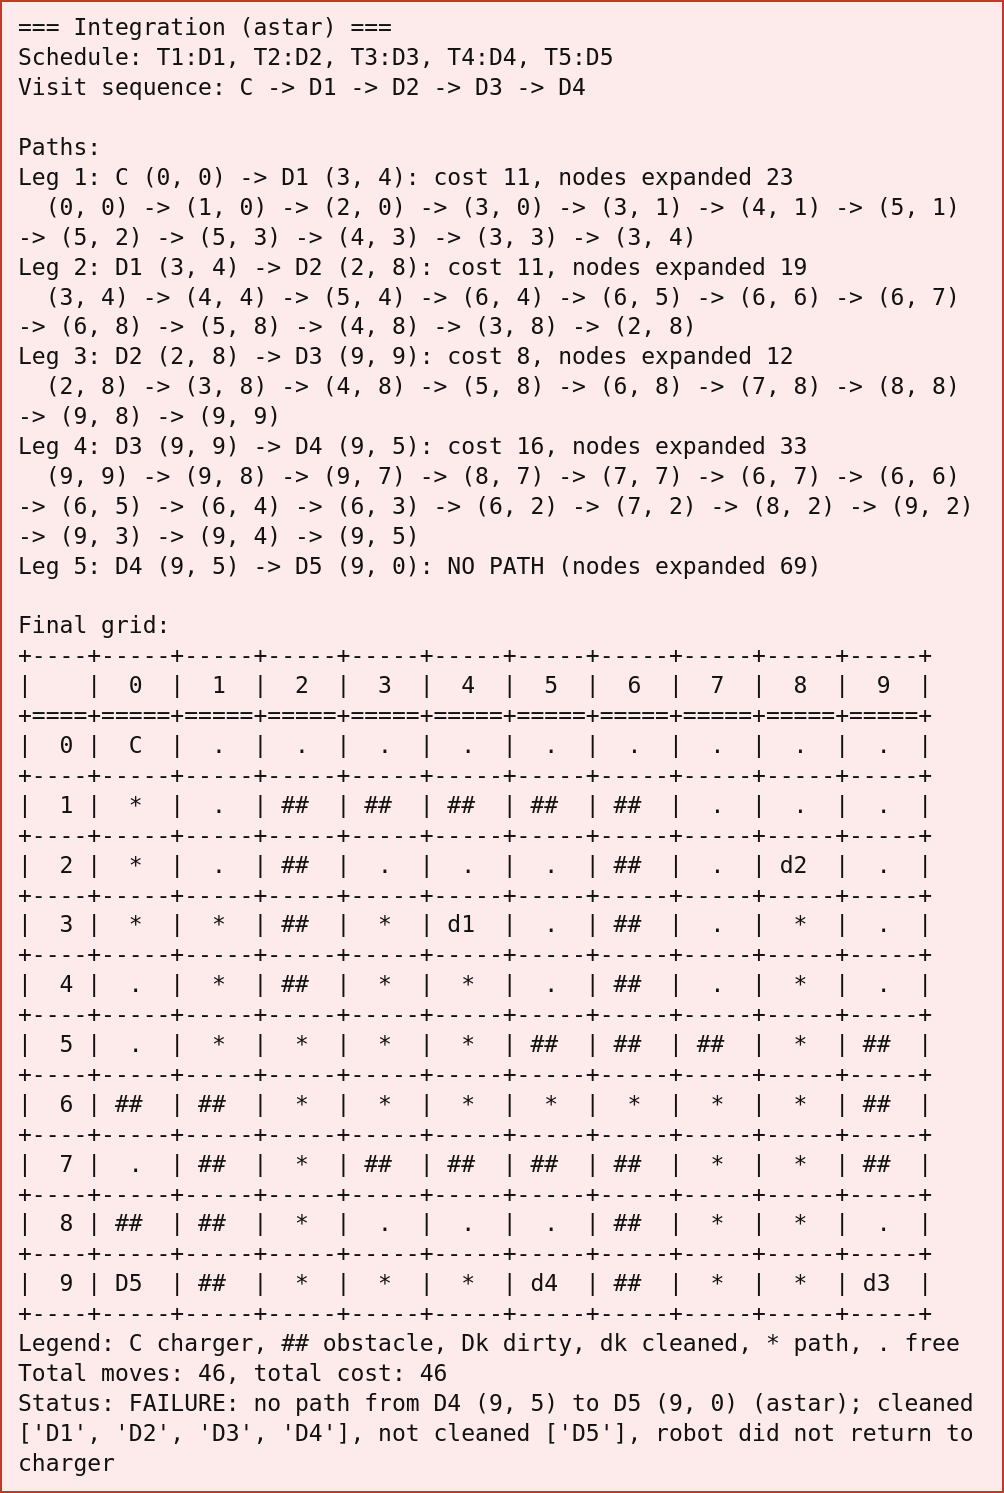
\includegraphics[width=0.8\linewidth]{run3_astar.png}
\caption{Test run 3 (error files): integration output with \astar.}
\label{fig:run3-astar}
\end{figure}
\figcenterend


\newpage
\subsection{Automated tests}
{\emergencystretch=3em In addition to the three runs, \code{pytest} runs 94 tests (all passing).
They cover the parsers (valid files, the sample files, and each invalid-input rule), successors,
path cost, the heuristic and both search algorithms (including start $=$ goal and no path; costs on
many start/goal pairs of our grid are checked against a breadth-first-search distance), the CSP
functions (checked against a brute-force solver that tries every assignment), integration (success,
an unreachable leg, an infeasible schedule) and the display. A seeded generator
(\code{tools/gen\_env.py}) produces random reachable/unreachable environments and
feasible/infeasible schedules; property-based tests (Hypothesis) check that the generated files
parse and have the requested properties. Continuous integration runs lint, tests, robustness,
interface checks, and a full execution of the notebook on every pull request.\par}
